\chapter{Marco teórico}

\section{Ecuaciones y citarlas}

\begin{comment}
  Objetivo: Explicarles a los lectores de computación que entienden
  los lingüistas de una variación dialectal
\end{comment}

Divergencia de $\vec{u}$ \eqref{eq:divergence}, ecuación de Navier-Stokes \eqref{eq:NavierStokes}. La \cref{tab:dielectricK}

Citar usando cref:

En las \cref{fig:Cpx_rans_8,fig:Cpx_rans_10} , las \cref{eq:divergence,eq:NavierStokes} En la  \cref{tab:dielectricK}... En el \cref{c:codigo}

\begin{equation}\label{eq:divergence}
    \nabla\cdot \vec{u}
\end{equation}

\begin{equation}\label{eq:NavierStokes}
\frac{\partial \bar{u_i}}{\partial t} +\bar{u_j}\frac{\partial \bar{u_i}}{\partial x_j}=-\frac{1}{\rho}\frac{\partial \bar{p}}{\partial x_i}+\nu\frac{\partial^2 \bar{u_i}}{\partial x_j^2}+\frac{f_b}{\rho}
\end{equation}

Dividir una ecuación larga usando dmath del paquete breqn:

\begin{dmath}\label{eq:reynolds:_transport}
\frac{\partial}{\partial t}\left \langle u_i u_k\right \rangle+U_j\frac{\partial}{\partial x_j}\left \langle u_i u_j\right \rangle = \frac{p}{\rho}\left[\frac{\partial u_i}{\partial x_k}+\frac{\partial u_k}{\partial x_i} \right]+\frac{\partial}{\partial x_j}\left \{ -\frac{1}{\rho}\left[ \left \langle pu_k\right \rangle\delta_{ij}+\left \langle pu_i\right \rangle\delta_{kj}\right] -\left \langle u_i u_j u_k\right \rangle+ 2\nu\left [ s_{ij}u_k+s_{ikj}u_i \right ] \right \}-\left [ u_i u_j \frac{\partial U_k}{\partial x_j}+u_k u_j \frac{\partial U_i}{\partial x_j} \right ]-2\nu\left [ s_{ij} \frac{\partial u_k}{\partial x_j}+s_{kj}\frac{\partial u_i}{\partial x_j} \right ]
\end{dmath}

\subsection{Unidades con el paquete siunitx}

La gravedad tiene una aceleración de \SI{9.8}{ms^{-2}},\\
\si{\kilo\gram\metre\per\square\second} \\
\si{\gram\per\cubic\centi\metre}\\        \si{\square\volt\cubic\lumen\per\farad}\\
\si{\metre\squared\per\gray\cubic\lux} \\ 
\si{Hs}\\
\SI{200}{GHz}

Para mas detalles consultar \href{https://ctan.mirrors.hoobly.com/macros/latex/contrib/siunitx/siunitx.pdf}{Manual de usuario de siunitx}.

\subsection{Citar una referencias}

Diferentes formas de citar a una referencia o autor \citet{abdollahzadeh2016implementation}, Suzen \cite{suzen_numerical_2005} y citar el año de publicación del trabajo \citeyear{dorr_numerical_2015}:

\section{Tablas}



Ejemplo de una Tabla \ref{tab:dielectricK}.

\begin{table}[!ht]
\centering
\caption{Permitividad relativa de diferentes dieléctricos}
\label{tab:dielectricK}
\begin{tabular}{@{}cc@{}}
\toprule
Material           & Permitividad Relativa ($\varepsilon_r$)\\ \midrule
Aire               & 1.0                   \\
Kapton (Poliimida) & 3.4                   \\
Plexiglas          & 4.7                   \\
Teflón             & 2.7                   \\
Vidrio             & 6.7                   \\ \bottomrule
\end{tabular}
\end{table}

\section{Figuras}

Una figura simple \ref{fig:Cpx_rans_14}. Las subfiguras, se pueden citar individualmente  y \ref{fig:Cpx_rans_10} o en su conjunto \ref{fig:Cpx_rans_a2}.

\begin{figure}[ht!]
  \centering
    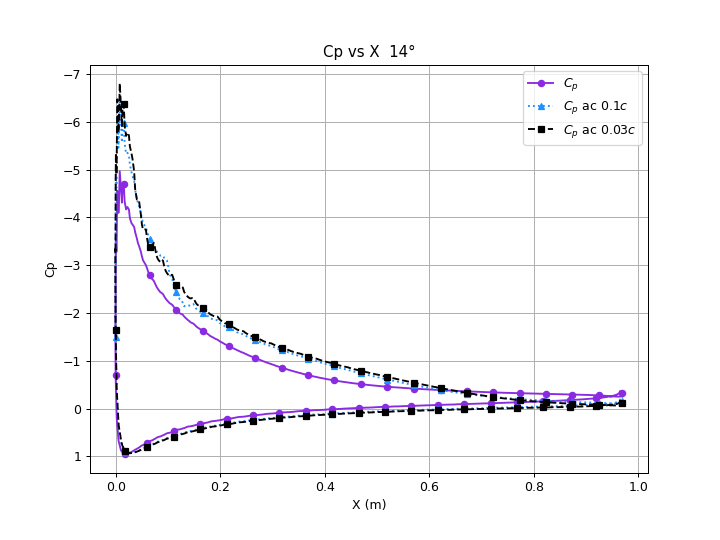
\includegraphics[width=0.75\textwidth]{Cpx_rans_14}    
    \caption{Distribución de coeficientes de presión.}         
  \label{fig:Cpx_rans_14}                          
\end{figure}


\begin{figure}[ht!]
\centering
\begin{subfigure}{0.5\textwidth}
  \centering
  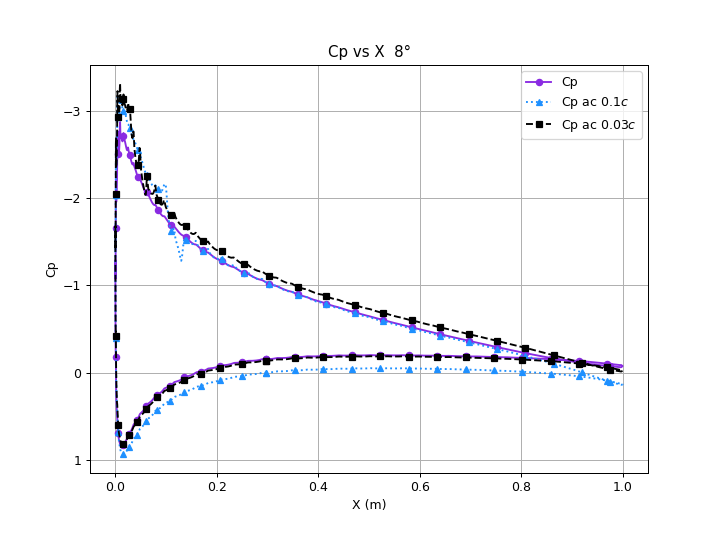
\includegraphics[width=1.0\textwidth]{Cpx_rans_8}
  \caption{Distribución de Cp para $\alpha=8^\circ$.}
  \label{fig:Cpx_rans_8}
\end{subfigure}%
\begin{subfigure}{0.5\textwidth}
  \centering
  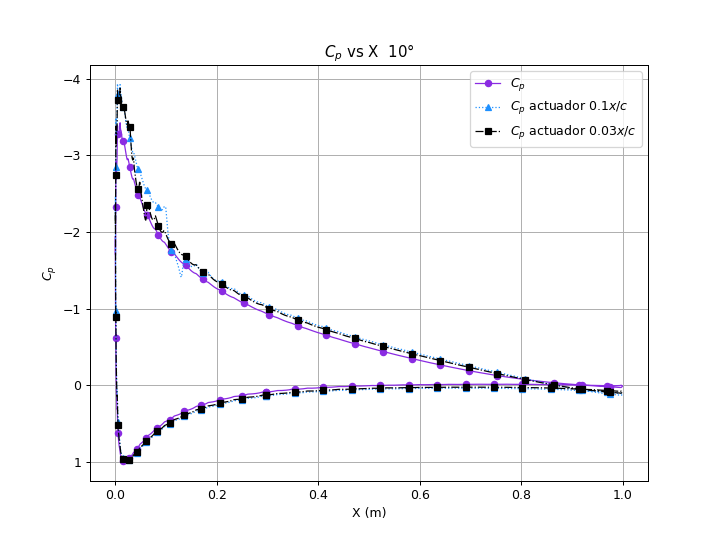
\includegraphics[width=1.0\textwidth]{Cpx_rans_10}
  \caption{Distribución de Cp para $\alpha=10^\circ$.}
  \label{fig:Cpx_rans_10}
\end{subfigure}
\caption{Distribución de presión sobre la superficie del perfil.}
\label{fig:Cpx_rans_a2}
\end{figure}    

\subsection{Arboles de directorios}

Es posible crear arboles de directorios:

\dirtree{%
.1 icoFoam.
.2 Make.
.3 files.
.3 options.
.2 createFields.H.
.2 icoFoam.C.
}
